\documentclass[a4paper,10pt]{article}


\usepackage{tikz}
\usepackage{graphicx}
\usepackage{url}
\usepackage[top=1.0in, bottom=1.0in, left=.6in, right=.6in]{geometry}
\usepackage{float}
\addtolength{\topmargin}{-.50in}
\title{Pushdown automaton criterion for completeness of coverability sets}
\author{Vipul Harsh \and J\'er\^ome Leroux \and Gr\'egoire Sutre\\
        IIT Bombay , INDIA\\
        \texttt{vipulharsh.cse.iitb.ac.in}\\[0.3 cm]
        }



% Natural numbers
\usepackage{amssymb,amsmath}
\newcommand{\setN}{\mathbb{N}}

% Vectors
\def\vec#1{\mathchoice{\mbox{\boldmath$\displaystyle#1$}}
{\mbox{\boldmath$\textstyle#1$}}
{\mbox{\boldmath$\scriptstyle#1$}}
{\mbox{\boldmath$\scriptscriptstyle#1$}}}


\begin{document}


\maketitle

The set of natural numbers $\setN$ is extended with a special symbol $\omega\not\in\setN$. The completed set $\setN\cup\{\omega\}$ is denoted by $\setN_\omega$. The sum function is extended over $\setN_\omega$ by $x+y=\omega$ if $x=\omega$ or $y=\omega$. The classical total order $\leq$ over $\setN$ is extended into the total order over $\setN_\omega$, still denoted by $\leq$, and defined by $x\leq y$ if, and only if, there exists $z\in\setN_\omega$ such that $y=x+z$. In the sequel, $d$ denotes a natural number, called the \emph{dimension}. The sum and the total order are also extended component-wise over the vectors in $\setN_\omega^d$.


\medskip

A \emph{Petri net} is a finite set $T$ of pairs in $\setN^d\times\setN^d$. Pairs $t\in\setN^d\times\setN^d$ are called \emph{transitions}, and vectors in $\setN_\omega^d$ are called \emph{configurations}. We associate to every transition $t$ given as a pair $(\vec{a},\vec{b})\in\setN^d\times\setN^d$ the binary relation $\xrightarrow{t}$ over the configurations defined by $\vec{x}\xrightarrow{t}\vec{y}$ if, and only if, $\vec{x}\geq \vec{a}$, $\vec{y}\geq \vec{b}$, and $\vec{x}+\vec{b}=\vec{y}+\vec{a}$. A finite set $\vec{C}\subseteq \setN_\omega^d$ is said to be \emph{closed} for the Petri net $T$ if for every $\vec{c}\xrightarrow{t}\vec{y}$ with $\vec{c}\in\vec{C}$ and $t\in T$, there exists $\vec{c}'\in\vec{C}$ such that $\vec{y}\leq \vec{c}'$.


\medskip


Given a word $\sigma=t_1\ldots t_k$ of transitions $t_j\in T$, we denote by $\xrightarrow{\sigma}$ the binary relation over the configurations defined by $\vec{x}\xrightarrow{\sigma}\vec{y}$ if, and only if, there exists a sequence $\vec{c}_0,\ldots,\vec{c}_k$ of configurations such that $\vec{c}_0=\vec{x}$, $\vec{c}_k=\vec{y}$ and such that $\vec{c}_{j-1}\xrightarrow{t_j}\vec{c}_j$ for every $1\leq j\leq k$. We also denote by $\xrightarrow{\sigma^\omega}$ the binary relation over the configurations defined by $\vec{c}\xrightarrow{\sigma^\omega}\vec{c}'$ if there exists a configuration $\vec{y}\geq \vec{c}$ such that $\vec{c}\xrightarrow{\sigma}\vec{y}$ and such that $\vec{c}'(i)=\vec{c}(i)$ if $\vec{c}(i)=\vec{y}(i)$ and $\vec{c}'(i)=\omega$ if $\vec{c}(i)<\vec{y}(i)$ for every $1\leq i \leq d$.


\medskip


An \emph{accelerated graph} for a Petri net $T$ is a tuple $G=(Q,\Lambda,\Delta,\Delta_\omega,\sqsubseteq)$ where $Q$ is a finite set of \emph{states}, $\Lambda:Q\rightarrow\setN_\omega^d$, $\Delta$ is a finite set of triples $(q,t,q')\in Q\times T\times Q$ such that $\Lambda(q)\xrightarrow{t}\Lambda(q')$, $\Delta_\omega$ is a finite set of triples $(q,\sigma,q')\in Q\times T^*\times Q$ such that $\Lambda(q)\xrightarrow{\sigma^\omega}\Lambda(q')$, and $\sqsubseteq$ is a binary relation over $Q$ satisfying $q\sqsubseteq q'\Rightarrow\Lambda(q)\leq \Lambda(q')$. Given a finite set $Q'\subseteq Q$, we are intereted in a sufficient condition, given as a pushdown automaton, such that $\vec{C}=\{\Lambda(q') \mid q'\in Q'\}$ is closed for $T$.



\section{Introduction}
  Consider a set of nodes , S for which we need to check completeness for a given Petri Net P. Also , consider 
  another set I of nodes.
  We aim to construct a pushdown automaton $\xi$  to verify the completness of the set S as the coverability 
  set for P.  
  
\section{Construction}
  \subsection{Start State} 
    There is only one start state labelled "Start".
    \newline
    \begin{center}
    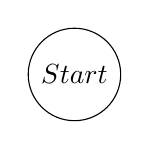
\begin{tikzpicture}
            \node[circle,draw] (q0) at (0,-1) {$Start$};
    \end{tikzpicture}
    \end{center}
    
  \subsection{Set of States}
    The set of states comprise of the following
    \begin{enumerate}
      \item  The start state (discussed in the earlier section)
      \item  The set of states - S
      \item  The set of states - I
    \end{enumerate}
      
   \subsection{Acceptance and Final states}
     A word is accepted if a run on the word ends in an empty stack and a state belonging to the set S.
     Thus , the set of final states is S and acceptance is by empty stack.
     
   \subsection{Input Alphabet}
     The input alphabet is the set of nodes(their names/symbols) belonging to set S and the set of transitions of the Petri Net P.
   
   \subsection{Stack Alphabet}
     The set of Transitions(their names/symbols).
     
   
   \subsection{Transitions}
   \begin{enumerate}
      
     %1 
      \item  From the start state, for every node alphabet(i.e. alphabets which represent nodes in S),
            We have a transition from the start state to the node represented by the alphabet. 
            No change is affected in the stack. 
      \begin{center}
      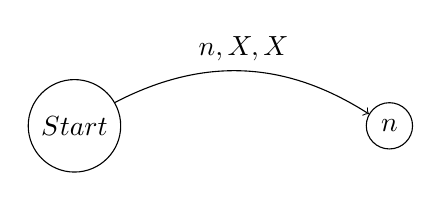
\begin{tikzpicture}
        \node[circle,draw] (q0) at (0,-1) {$Start$};
        \node[circle,draw] (q1) at (4,-1) {$n$};
        \draw[->] (q0) edge[bend left] node[above] {$n,X,X$} (q1);
        \end{tikzpicture}

      \end{center}
      These are the only transitions from the start state. 
      \newline
      Also after this point ,in our context we do not expect any input letters from the 
      alphabets representing nodes in S.
      
      
     %2 
      \item
      The label of n2 is exactly n1 + Action(t). 
      \begin{itemize}
        \item The transition from n1 to n2 : t is popped out from the stack. Nothing is pushed.
        \item The transition from n2 to n1 : t is pushed to the stack. Nothing is popped.
      \end{itemize}
      \begin{center}
      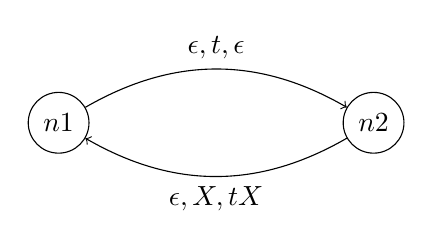
\begin{tikzpicture}
        \node[circle,draw] (q0) at (0,-1) {$n1$};
        \node[circle,draw] (q1) at (4,-1) {$n2$};
        \draw[->] (q0) edge[bend left] node[above] {$\epsilon ,t,\epsilon $} (q1);
        \draw[->] (q1) edge[bend left] node[below] {$\epsilon ,X,tX $} (q0);
        \end{tikzpicture}

      \end{center}
        
   
   %3
   \item
      The label of n2  $\geq$ n1 . No change is affected in the stack in this case. 
      \begin{center}
      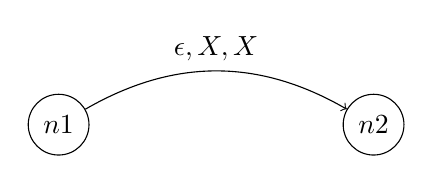
\begin{tikzpicture}
        \node[circle,draw] (q0) at (0,-1) {$n1$};
        \node[circle,draw] (q1) at (4,-1) {$n2$};
        \draw[->] (q0) edge[bend left] node[above] {$\epsilon ,X,X$} (q1);
        \end{tikzpicture}

      \end{center} 
   
   
   
   
   
   
   
   
   
   
   
   
   
   %4
   
   \item
      The label of n2 is n1 + Action(t), with extra $\Omega$ in some places. 
      
      \begin{center}
      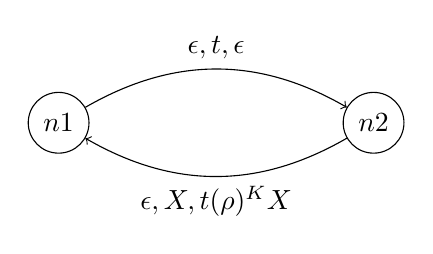
\begin{tikzpicture}
        \node[circle,draw] (q0) at (0,-1) {$n1$};
        \node[circle,draw] (q1) at (4,-1) {$n2$};
        \draw[->] (q0) edge[bend left] node[above] {$\epsilon ,t,\epsilon $} (q1);
        \draw[->] (q1) edge[bend left] node[below] {$\epsilon ,X,t(\rho)^{K} X $} (q0);
        
        \end{tikzpicture}

      \end{center}
       Where $\rho$ $\in$ $T^{\ast}$ \& Action($\rho$) yields positive tokens in the 
       places where $\Omega$ are put and 0 elsewhere , \newline 
       for all K $\geq$ $K_{0}$ (for a given $K_{0}$).
       \newline
       T is the set of transitions. 
      
       \end{enumerate}
   
   
   \subsection{Initial Stack Alphabet}
    Initially , the stack is empty.    

    
    
\end{document}

